Рассматриваем задачу оптимизации суммы большого количества функций:
\begin{gather*}
    F(x) = \dfrac{1}{n} \sum\limits_{i=1}^{n} \, f_{i} (x) \to \min\limits_{x}, \quad f_{i} \in C^{1}, \quad n \gg 1 \\
    \nabla F(x) = \dfrac{1}{n} \sum\limits_{i=1}^{n} \, \nabla f_{i} (x)
\end{gather*}
Рассмотрим стоимости вычисления различных величин:
\begin{center}
    \begin{tabular}{|c|c|}
        \hline
        Величина       & Стоимость вычисления \\
        \hline
        $f_{i}(x)$        & $O(q)$               \\
        \hline
        $\nabla f_{i}(x)$ & $O(q)$               \\
        \hline
        $F(x)$            & $O(nq)$              \\
        \hline
        $\nabla F(x)$     & $O(nq)$              \\
        \hline
    \end{tabular}
\end{center}
Вычисляем функции $f_{i}(x)$ через граф вычислений, градиент это обратный проход по графу - стоимость та же. Видим, что стоимость вычисления оракулом функции $F$ и её градиента линейно зависит от размера выборки. Хотим метод, у которого стоимость итерации не будет зависеть от размера выборки.

\subsubsection{SGD (стохастический градиентный метод)}
Посмотрим на одну итерацию метода:
\begin{algorithmic}[1]
    \Procedure{SGD}{}
        \State $i_k \gets \textsc{UNIFORM}(1, 2, \dots , n) \quad \left(O(1)\right)$
        \State $g_k \gets \nabla f_{i_{k}}(x_k) \quad \left(O(q)\right)$
        \State $x_{k+1} \gets x_k - \alpha_k g_k \quad \left(O(d)\right)$
    \EndProcedure
\end{algorithmic}
Стоимость итерации $O(q)$. Видно, что $g_k$ является несмещенной оценкой для $\nabla F(x)$:
\[
    \mathbb{E}_{i \sim \textsc{UNIFORM}} \, g_k = \dfrac{1}{n} \sum\limits_{i=1}^{n} \, \nabla f_{i}(x) = \nabla F(x)
\]
Также можно сэмплировать не один индекс, а какое-то множество индексов фиксированного размера:
\begin{algorithmic}[1]
    \Procedure{SGD + mini-batches}{}
        \State $I_k \subset \textsc{UNIFORM}(1, 2, \dots , n) \quad \left(O(|I_k|)\right)$
        \State $g_k \gets \dfrac{1}{|I_k|} \sum\limits_{i_k \in I_k} \, \nabla f_{i_{k}}(x_k) \quad \left(O(q|I_k|)\right)$
        \State $x_{k+1} \gets x_k - \alpha_k g_k \quad \left(O(d)\right)$
    \EndProcedure
\end{algorithmic}
Очевидно, что это тоже несмещенная оценка. Дисперсия стохастической оценки падает как $O(\dfrac{1}{\sqrt{k}})$, а увеличение стоимости происходит как $O(k)$. Таким образом выгодно использовать именно маленькие батчи. \\
Хотим посмотреть как будет работать стохастический градиент, приведем пример одномерного случая:
\[
    F(w) = \dfrac{1}{n} \sum\limits_{i=1}^{n} \underbrace{(y_i - wx_i)^2}_{f_i(w)} \to \min\limits_{w \in \mathbb{R}}
\]
\begin{figure}[h]
    \center
    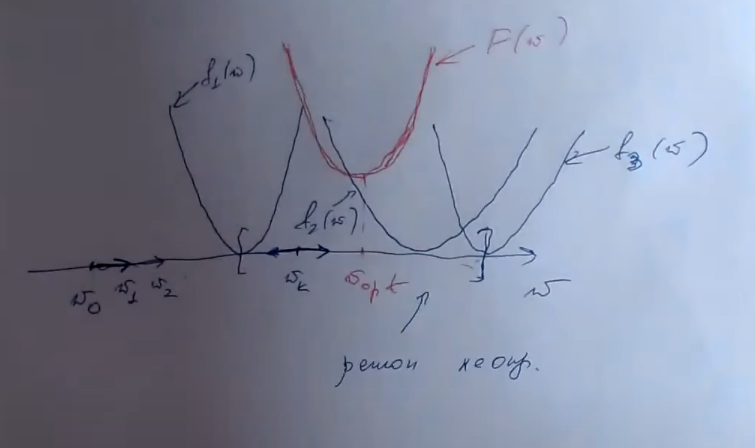
\includegraphics[width=10cm]{images/sgd.png}
\end{figure}
\\
Метод стохастического градиентного спуска вообще не является методом спуска, мы не гарантируем, что на каждой итерации значение функции уменьшится. Видно, что подходя к оптимуму мы попадаем в регион неопределенности, ведь даже в оптимальной точке наша оценка градиента $g_k$ не равна нулю, как нам того хотелось бы. Метод застревает около оптимума и начинает бесконечные колебания. У нас нет возможности оценить значение функции $F$, таким образом мы можем просто запускать метод на какое-то фиксированное число итераций, либо по каким-то косвенным признакам отслеживать (допустим в машинном обучении смотреть качество на отложенной выборке). В дальнейшем мы рассмотрим решение этой проблемы с помощью выбора длины шага и вариаций оценки градиента. Пока же предлагается оценить сходимость метода SGD.

\subsubsection{Скорость сходимости}
\[
    x_{k+1} = x_k - \alpha_k g_k, \quad \mathbb{E} \, g_k = \nabla F(x_k)
\]
Начинаем с невязки по точкам:
\[
    \| x_{k+1} - x_* \|^2 = \| x_k - \alpha_k g_k - x_* \|^2 = \| x_k - x_* \|^2 - 2\alpha_k g_k^T (x_k - x_*) + \alpha_k^2 \| g_k \|^2
\]
Теперь берем матожидание по случайности на $k-$ой итерации:
\[
    \mathbb{E}_{i_{k}} :\quad  \mathbb{E}_{i_{k}} \| x_{k+1} - x_* \|^2 = \| x_k - x_* \|^2 - 2\alpha_k \nabla F(x_k)^T (x_k - x_*) + \alpha_k^2 \mathbb{E}_{i_{k}} \| g_k \|^2
\]
Предполагаем, что $F$ - выпуклая функция, тогда:
\begin{gather*}
    F(x_*) \geq F(x_k) + \nabla F(x_k)^T (x_* - x_k) \\
    F(x_k) - F(x_*) \leq \nabla F(x_k)^T (x_k - x_*)
\end{gather*}
Теперь:
\[
    \alpha_k \nabla F(x_k)^T (x_k - x_*) = \dfrac{\| x_k - x_* \|^2}{2} + \dfrac{\alpha_k^2 \mathbb{E}_{i_{k}} \| g_k \|^2}{2} - \dfrac{\mathbb{E}_{i_{k}} \| x_{k+1} - x_* \|^2}{2}
\]
\[
    \alpha_k (F(x_k) - F(x_*)) \leq \dfrac{\| x_k - x_* \|^2}{2} + \dfrac{\alpha_k^2 \mathbb{E}_{i_{k}} \| g_k \|^2}{2} - \dfrac{\mathbb{E}_{i_{k}} \| x_{k+1} - x_* \|^2}{2}
\]
Теперь давайте возьмем матожидание по всей случайности:
\[
    \mathbb{E}: \quad \alpha_k (\mathbb{E} F(x_k) - F(x_*)) \leq \dfrac{\mathbb{E} \| x_k - x_* \|^2}{2} + \dfrac{\alpha_k^2 \mathbb{E} \| g_k \|^2}{2} - \dfrac{\mathbb{E} \| x_{k+1} - x_* \|^2}{2}
\]
Теперь просуммируем по индексам от $0$ до $k$:
\[
    \sum\limits_{i=0}^{k} \alpha_i (\mathbb{E} F(x_i) - F(x_*)) \leq \dfrac{\| x_0 - x_* \|^2}{2} + \dfrac{\sum\limits_{i=0}^{k} \alpha_i^2 \mathbb{E} \| g_i \|^2}{2} - \dfrac{\mathbb{E} \| x_{k+1} - x_* \|^2}{2}
\]
Вспоминаем, что $F$ - выпуклая, записываем неравенство Йенсена:
\[
    \mathbb{E} F\left(\overbrace{\dfrac{\sum\limits_{i=0}^{k} \alpha_i x_i}{\sum\limits_{i=0}^{k}\alpha_i}}^{\overline{x_k}}\right) - F(x_*) \leq \dfrac{\sum\limits_{i=0}^{k} \alpha_i (\mathbb{E} F(x_i) - F(x_*))}{\sum\limits_{i=0}^{k}\alpha_i} \leq \dfrac{\| x_0 - x_* \|^2 + \sum\limits_{i=0}^{k} \alpha_i^2 \mathbb{E} \| g_i \|^2}{2\sum\limits_{i=0}^{k}\alpha_i}
\]
Теперь ограничим начальную невязку как $R^2$, положим, что все $f_i \in C^{0, 0}_{G}$, тогда можно ограничить норму квадрата градиента как $G^2$:
\[
    \mathbb{E} F(\overline{x_k}) - F(x_*) \leq \dfrac{R^2 + G^2 \sum\limits_{i=0}^{k} \alpha_i^2}{2\sum\limits_{i=0}^{k}\alpha_i}
\]
Таким образом с точки зрения теоремы мы можем гарантировать что-либо только для средней точки $\overline{x_k}$, однако "если провести численные эксперименты, мы увидим, что разница не существенная". \\
Теперь рассмотрим разные стратегии выбора длины шага $\alpha_k$:

\subsubsection{Стратегии выбора длины шага}
\begin{itemize}
    \item \textbf{Константный} $\alpha_k = h$:
    \[
        \dfrac{R^2 + G^2 h^2 (k+1)}{2(k+1)h} = \dfrac{R^2}{2h(k+1)} + \dfrac{G^2 h}{2} \to_{k \to \infty} \dfrac{G^2 h}{2}
    \]
    \begin{figure}[h]
        \center
        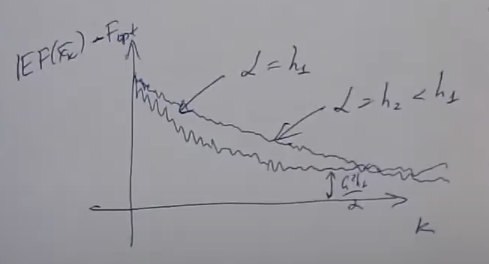
\includegraphics[width=7cm]{images/sgd2.png}
    \end{figure}
    \\
    Видно, что при меньшем шаге мы сходимся медленнее, зато в меньшее значение невязки.
    Однако это всё про матожидание, и тут на помощь нам приходит неравенство Маркова:
    \[
        \xi := F(\overline{x_k}) - F(x_*) \geq 0 \Rightarrow p\left( F(\overline{x_k}) - F(x_*) \geq a \right) \leq \dfrac{\mathbb{E}F(\overline{x_k}) - F(x_*)}{a}
    \]
    \item \textbf{Устремить к нулю $\alpha$}
    \begin{enumerate}
        \item $\sum\limits_{i=0}^{k} \alpha_i = \infty, \ \ \sum\limits_{i=0}^{k} \alpha_i^2 < \infty$
        \[
            \alpha_i = \dfrac{h}{(i + 1)^{\tau}}, \quad \tau \in \left(\dfrac{1}{2}, 1\right]
        \]
        \item $\sum\limits_{i=0}^{k} \alpha_i = \infty, \ \ \sum\limits_{i=0}^{k} \alpha_i^2 = \infty, \ \ \lim\limits_{k \to \infty}\dfrac{\sum\limits_{i=0}^{k} \alpha_i^2}{\sum\limits_{i=0}^{k} \alpha_i} = 0$
        \[
            \alpha_i = \dfrac{h}{(i + 1)^{\tau}}, \quad \tau \in \left(0, \dfrac{1}{2}\right]
        \]
    \end{enumerate}
    $\tau_{opt} = \dfrac{1}{2} \Rightarrow$ скорость сходимости будет $O\left(\dfrac{\ln(k)}{\sqrt{k}}\right) = \tilde{O}\left(\dfrac{1}{\sqrt{k}}\right)$.
\end{itemize}
Составим табличку скоростей сходимости методов и их стохастических аналогов:
\begin{center}
{\renewcommand{\arraystretch}{1.4}
\begin{tabular}{|c|c|c|c|}
    \hline
    & & \multicolumn{2}{|c|}{Скорость сходимости} \\
    \hline
    Метод          & Функция                               & Обычный                     & Стохастический              \\
    \hline
    Градиентный    & $f \in C^{1,1}_{L}$ и сильно выпуклая & $O(C^k)$                    & $O(\nicefrac{1}{k})$        \\
    \hline
    Градиентный    & $f \in C^{1,1}_{L}$ и выпуклая        & $O(\nicefrac{1}{k})$        & $O(\nicefrac{1}{\sqrt{k}})$ \\
    \hline
    Субградиентный & $f \in C^{0,0}_{L}$ и выпуклая        & $O(\nicefrac{1}{\sqrt{k}})$ & $O(\nicefrac{1}{\sqrt{k}})$ \\
    \hline
\end{tabular}
}
\end{center}
Видно, что с такой скоростью сходимости для требуемой точности необходимо огромное число итераций, хотим метод с линейной скоростью сходимости.

\subsubsection{SAG и SVRG}

\paragraph{SAG}
\begin{gather*}
    \textsc{GD}: \quad x_{k+1} = x_k - \alpha_k \dfrac{1}{n} \sum\limits_{i=1}^{n} \nabla f_i (x_k) \\
    \textsc{SAG}: \quad x_{k+1} = x_k - \alpha_k \dfrac{1}{n} \sum\limits_{i=1}^{n} \nabla f_i (v_i^k)
\end{gather*}
Пытаемся сделать так, чтобы в пределе направление оптимизации приходило в полный градиент. На каждой итерации меняем одну точку $v_i^k$. Рассмотрим итерацию метода:
\begin{algorithmic}[1]
    \Procedure{SAG}{}
        \State $i_k \gets \textsc{UNIFORM}(1, 2, \dots , n)$
        \State $v_{i_k}^k \gets x_k; v_{j}^k \gets v_{j}^{k-1} \, \forall j \neq i_k $
        \State $g_k \gets \dfrac{1}{n} \sum\limits_{i=1}^{n} \nabla f_i (v_i^k) = g_{k-1} + \dfrac{1}{n} \left(\nabla f_{i_k}(v_{i_k}^k) - \nabla f_{i_k}(v_{i_k}^{k-1})\right)$
        \State $x_{k+1} \gets x_k - \alpha_k g_k$
    \EndProcedure
\end{algorithmic}
В методе возникает память, которая имеет размер, зависящий от количества объектов: $O(nd)$. \\
Для скорости сходимости метода SAG верно следующее утверждение (оно вида теоремы, но главный по оптам сказал можно не доказывать и даже не формулировать строго):
\theorem{
Пусть $F \in C^{1,1}_{L}$ и $\mu$ сильно выпуклая, длина шага $\alpha_k = \dfrac{1}{16L}$, тогда для невязки по функции для метода SAG верна следующая оценка:
\[
    \mathbb{E} F(x_k) - F(x_*) \leq \left( 1 - \min\left( \dfrac{\mu}{16L}, \dfrac{1}{8n} \right) \right)^k C
\]
}
Имеет обратить внимание на то, что $k$ - это номер стохастической итерации, то есть он сходится быстрее градиентного спуска где-то в $n$ раз. Также у него есть возможность адаптивного подбора константы Липшица.\\
Однако он работает только для выпуклых и сильно выпуклых функций. И еще стоит обратить внимание в связи с этим методом, на то, что он оптимизирует именно сумму функций и направлен на это. То есть в более общем случае, когда мы оптимизируем функцию вида матожидание по распределению мы не можем использовать SAG:
\[
    F(x) = \mathbb{E}_{q(y)} f(x, y) \to \min\limits_{x}
\]
Ну и далее мы рассмотрим метод, похожий на SAG, однако который можно применять на более общие задачи вида выше.

\paragraph{SVRG}
Идея следующая, в какой-то точке потратить время и посчитать полный градиент функции, потом использовать его для построения оценок для $g_k$:
\begin{gather*}
    \tilde{x}: \quad \tilde{\mu} = \dfrac{1}{n} \sum\limits_{i=1}^{n} \nabla f_i (\tilde{x}) = \nabla F(\tilde{x}) \\
    g_k = \nabla f_{i_k} (x_k) - \nabla f_{i_k} (\tilde{x}) + \tilde{\mu} \\
    \mathbb{E} g_k = \mathbb{E} \nabla f_{i_k} (x_k) - \mathbb{E} \nabla f_{i_k} (\tilde{x}) + \mathbb{E} \tilde{\mu} = \nabla F(x_k)
\end{gather*}
Таким образом мы в методе совершаем итерации вида: оцениваем полный градиент в точке $\tilde{x_0}$, делаем какое-то количество стохастических итераций, оцениваем полный градиент в точке $\tilde{x_1}$ и так далее. Его можно применять для общих функций вида матожидание по распределению, у него есть теорема аналогичная как для SAG, что он сходится линейно с константным шагом обратно пропорциональным константе Липшица, у него есть критерий останова связанный с нормой $\tilde{\mu}$ и у него есть возможность адаптивного подбора константы Липшица, то есть его можно запускать что называется "из коробки".